\chapter{Shannon entropy}
\lbl{ch:shannon}

\begin{quote}
My greatest concern was what to call it. I thought of calling it
`information', but the word was overly used, so I decided to call it
`uncertainty'.  When I discussed it with John von Neumann, he had a better
idea.  Von Neumann told me, `You should call it entropy, for two
reasons. In the first place your uncertainty function has been used in
statistical mechanics under that name, so it already has a name.  In the
second place, and more important, no one knows what entropy really is, so
in a debate you will always have the advantage.'  
\hfill 
-- Claude Shannon%
%
\index{Shannon, Claude}%
\index{Neumann, John@von Neumann, John}
%
(quoted in~\cite{TrMc}, p.~180).
\end{quote}

Entropy appears in almost every branch of science.  The most casual
literature search quickly brings up works on entropy in
thermodynamics~\cite{Ferm}, quantum physics~\cite{PST}, communications
engineering~\cite{ShanMTC,SCBE}, information theory~\cite{MacKITI},
statistical inference~\cite{JaynWDWS,JaynPTL}, machine learning and
artificial intelligence~\cite{BoKoPe,Deng,Ratn}, malware
detection~\cite{BJS}, macroecology~\cite{Hart}, the quantification of
biological diversity~\cite{Magu}, biochemistry~\cite{MDV}, water network
engineering~\cite{GDS}, the theory of algorithms and
complexity~\cite{Gacs}, ergodic theory and dynamical
systems~\cite{Parr,Down}, algebraic dynamics~\cite{EvWa}, combinatorial
dynamics~\cite{ALM}, topological dynamics~\cite{AKM}, and climate
science~\cite{HaTe}.  (The references given are a random sample.)  The word
`entropy' has many meanings, all related, and is applied in more ways
still.

This chapter is an introduction to the simplest kind of entropy: the
Shannon entropy of a probability distribution on a finite set.  There are
several ways of interpreting Shannon entropy, and we develop two in depth.
The first is through coding theory (Section~\ref{sec:ent-coding}), an
interpretation that is very standard in the mathematical literature and
goes back to Shannon's seminal paper of 1948~\cite{ShanMTC}.  The second is
through the theory of diversity (Section~\ref{sec:ent-div}).  This is
much less well-known, and is one of the main themes of this book.

The single most important property of Shannon entropy is the chain rule,
which is a formula for the entropy of a composite distribution.  The major
theoretical goal of this chapter is to prove that Shannon entropy is
essentially the \emph{only} quantity that satisfies the chain rule.  To
that end, we begin by reviewing probability distributions and composition
of them (Section~\ref{sec:prob-fin}).  The chain rule itself is derived in
Section~\ref{sec:ent-defn}, along with other basic properties of Shannon
entropy, and is explained in terms of coding and diversity in the next
two sections.  In the final section, we prove the unique characterization
of Shannon entropy by the chain rule.


\section{Probability distributions on finite sets}
\lbl{sec:prob-fin}


Let $n \geq 1$.  A \demph{probability distribution}%
%
\index{probability distribution} 
% 
on the finite set $\{1, \ldots, n\}$ is an $n$-tuple $\p = (p_1, \ldots,
p_n)$ of real numbers $p_i \geq 0$ such that $\sum p_i = 1$.

Of the various interpretations of probability distributions, one will be
especially important for us.

\begin{example}
\lbl{eg:prob-eco}
Consider an ecological community\index{community} of living organisms
classified into $n$ 
species.  Let $p_i$ be the relative abundance of
the $i$th species, where 
`relative'\index{abundance!relative} 
means that the abundances have been normalized so that $\sum p_i
= 1$.  Then the probability distribution $\p = (p_1, \ldots, p_n)$ is a
model of the community, albeit a very crude one.

Some remarks are in order.  First, the distinction between
species\index{species} is 
inexact and sometimes arbitrary.  Mayden~\cite{Mayd} lists~24 inequivalent
ways of defining `species' (further discussed in Hey~\cite{Hey}).  The
difficulty is most acute for microbes, many of which have not been
classified into species at all.  In practice, for microbes, scientists
sequence the DNA of their sample and use software that applies a clustering
algorithm, thus automatically creating `species' according to a pre-chosen
(and somewhat arbitrary) level of genetic similarity.  We will find a way
through this difficulty in Chapter~\ref{ch:sim}.

Second, the meaning of `abundance'%
%
\index{abundance!meaning of} 
% 
is completely flexible.  In some contexts, it may be appropriate to simply
count individuals.  But when the organisms are of very different sizes, it
may be better to interpret the abundance of a species as the total mass of
the members of that species.  Or, for plants, the area of land covered by a
species may be a more appropriate measure than the number of individuals.

Third, as emphasized in the Introduction (p.~\pageref{p:general}), nothing
that we will say about `communities' or `species' is actually specific to
ecology: mathematically speaking, it is entirely general.
\end{example}

For $n \geq 1$, write 
\[
\Delta_n 
=
\bigl\{ \text{probability distributions on } \{1, \ldots, n\} \bigr\}.
\ntn{Deltan}
\]
Occasionally we will want to
include the case $n = 0$, and we put $\Delta_0 = \emptyset$.  The
\demph{support}\index{support} of $\p \in \Delta_n$ is
\[
\supp(\p) 
=
\bigl\{ 
i \in \{1, \ldots, n\} 
\such
p_i > 0 \}.
\ntn{supp}
\]
We say that $\p \in \Delta_n$ has \demph{full%
%
\index{full support} 
% 
support} if $\supp(\p) = \{1, \ldots, n\}$, and write
\[
\lbl{p:simp-int}
\Delta_n^\circ 
=
\{ \p \in \Delta_n
\such
p_i > 0 \text{ for all } i \}
\ntn{Deltano}
\]
for the set of probability distributions of full support.  Finally,
\[
\vc{u}_n = (1/n, \ldots, 1/n)
\ntn{un}
\]
denotes the \demph{uniform%
% 
\index{uniform distribution} 
% 
distribution} on $n$ elements.  Geometrically, $\Delta_n$ is the standard
$(n - 1)$-dimensional simplex\index{simplex}, $\Delta_n^\circ$ is its
interior, and $\vc{u}_n$ is its centre.

\begin{example}
Consider a community consisting of species numbered $1, \ldots, n$, with
relative abundance distribution $\p \in \Delta_n$.  Then $\supp(\p)$ is the
set of species that are actually present in the community, and $\p \in
\Delta_n^\circ$ if and only if every species is present.  (A typical
situation in which some species are absent is a longitudinal study: if the
same site is surveyed every year over several years, it may be that in some
years, not every species is present.)  The uniform distribution $\vc{u}_n$
represents the situation in which all species are equally common.
\end{example}

We now define a fundamental operation: composition of probability
distributions (Figure~\ref{fig:comp}).  

\begin{defn}
\lbl{defn:comp-dist}
Let $n, k_1, \ldots, k_n \geq 1$ and let 
\[
\w \in \Delta_n, 
\
\p^1 \in \Delta_{k_1}, \ 
\ldots, \ 
\p^n \in \Delta_{k_n}.
\]
Write $\p^i = (p^i_1, \ldots, p^i_{k_i})$.  The
\demph{composite%
%
\index{composition!probability distributions@of probability distributions}
% 
distribution} is
% 
\begin{align*}
\w \of (\p^1, \ldots, \p^n)     &
=
(w_1 p^1_1, \ldots, w_1 p^1_{k_1}, 
\ \ldots, \ 
w_n p^n_1, \ldots, w_n p^n_{k_n})       
\ntn{comp}      \\
&
\in
\Delta_{k_1 + \cdots + k_n}.
\end{align*}
\end{defn}

\begin{figure}
\centering
\lengths
\begin{picture}(120,44)(0,-1)
\cell{60}{23}{c}{\includegraphics[height=40\unitlength]{composite2}}
\cell{60}{35}{c}{$\vc{w}$}
\cell{60}{25}{c}{$\cdots\cdots$}
\cell{60}{10}{c}{$\cdots$}
\cell{41}{15}{c}{$\p^1$}
\cell{79}{15}{c}{$\p^n$}
\cell{41}{5}{c}{$\cdots$}
\cell{79}{5}{c}{$\cdots$}
% 
\cell{42}{28}{c}{$w_1$}
\cell{78}{28}{c}{$w_n$}
\cell{33}{9}{c}{$p^1_1$}
\cell{51}{9}{c}{$p^1_{k_1}$}
\cell{71}{9}{c}{$p^n_1$}
\cell{88}{9}{c}{$p^n_{k_n}$}
\cell{32}{-1}{b}{$w_1 p^1_1$}
\cell{50}{-1}{b}{$w_1 p^1_{k_1}$}
\cell{70}{-1}{b}{$w_n p^n_1$}
\cell{89}{-1}{b}{$w_n p^n_{k_n}$}
\end{picture}
\caption{Composition of probability distributions.}
\lbl{fig:comp}
\end{figure}


\begin{example}
\lbl{eg:comp-coin}
\index{coin!die-card@-die-card process}
% 
Flip a coin.  If it comes up heads, roll a die.\index{die}  If it comes up
tails, draw from a pack of cards.%
% 
\index{cards, playing}  
% 
Thus, the final outcome of the process is either a
number between~1 and~6 or a playing card.  There are, therefore, $6 + 52 =
58$ possible final outcomes.

Assuming that the coin toss, die roll, and card draw are all fair, the
probabilities of the $58$ possible outcomes are as shown in
Figure~\ref{fig:comp-coin}.
% 
\begin{figure}
\centering
\lengths
\begin{picture}(120,45)(0,-2)
\cell{60}{23}{c}{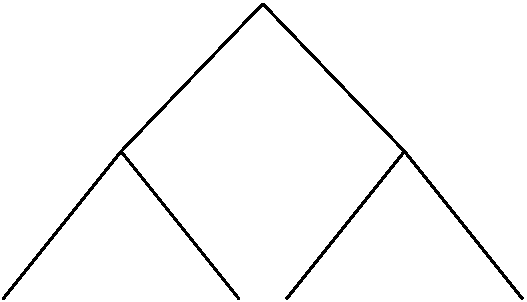
\includegraphics[height=40\unitlength]{coindiecards2}}
\cell{60}{30}{c}{Coin}
\cell{41}{12}{c}{Die}
\cell{79}{12}{c}{Cards}
\cell{41}{5}{c}{$\cdots$}
\cell{79}{5}{c}{$\cdots$}
% 
\cell{43}{29}{c}{$\hlf$}
\cell{77}{29}{c}{$\hlf$}
\cell{26}{9}{c}{$\tfrac{1}{6}$}
\cell{56}{9}{c}{$\tfrac{1}{6}$}
\cell{64}{9}{c}{$\tfrac{1}{52}$}
\cell{95}{9}{c}{$\tfrac{1}{52}$}
\cell{25}{-2}{b}{$\tfrac{1}{12}$}
\cell{56}{-2}{b}{$\tfrac{1}{12}$}
\cell{64}{-2}{b}{$\tfrac{1}{104}$}
\cell{94}{-2}{b}{$\tfrac{1}{104}$}
\end{picture}
\caption{The composite distribution of
  Example~\ref{eg:comp-coin}.} 
\lbl{fig:comp-coin}
\end{figure}
% 
That is, the final outcome has probability distribution
\[
\vc{u}_2 \of (\vc{u}_6, \vc{u}_{52}) 
=
\Bigl(
\underbrace{\tfrac{1}{12}, \ldots, \tfrac{1}{12}}_6, 
\underbrace{\tfrac{1}{104}, \ldots, \tfrac{1}{104}}_{52}
\Bigr).
\]
\end{example}

\begin{example}
\lbl{eg:comp-french}
\index{French language}
% 
The French language is written with the same letters as English, but some
are sometimes decorated by an accent (diacritical mark).  For instance, the
letter \as{a} appears in the three forms \as{a} (no accent), \as{\`{a}} and
\as{\^{a}}, the letter \as{b} appears only as \as{b}, and the letter \as{c}
appears in the two forms \as{c} and \as{\c{c}}.  Let us make the
conventions that a \demph{letter}\index{letter} is one of \as{a}, \as{b},
\ldots, \as{z} and a \demph{symbol}\index{symbol} is a letter together
with, optionally, an accent.  Thus, the symbols are \as{a}, \as{\`a},
\as{\^a}, \as{b}, \as{c}, \as{\c{c}}, \ldots

Let $\vc{w} \in \Delta_{26}$ denote the frequency distribution of the
letters as used in written French.  For the sake of argument, let us
suppose that $w_1, w_2, w_3, \ldots, w_{26}$ have the values shown in
Figure~\ref{fig:comp-french}.  Suppose also that the letter \as{a} appears
without accent 50\% of the time, as \as{\`a} 25\% of the time, and as
\as{\^a} 25\% of the time, again as in the figure.  Write $\p^1 = (0.5,
0.25, 0.25)$, and similarly for $\p^2, \ldots, \p^{26}$.  Then the
frequency distribution of the symbols is the composite
% 
\begin{multline*}
\vc{w} \of (\p^1, \ldots, \p^{26})\\
=
(0.05 \times 0.5, 0.05 \times 0.25, 0.05 \times 0.25, 0.02 \times 1, 
% 0.03 \times 0.5, 0.03 \times 0.5, 
\ldots, 0.004 \times 1).
\end{multline*}

\begin{figure}
\centering
\lengths
\begin{picture}(120,38)(-5,4)
\cell{55}{23}{c}{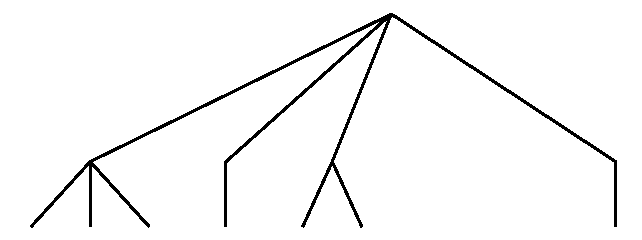
\includegraphics[height=42\unitlength]{accents_white_boxes}}
\cell{23}{22}{b}{\small 0.05}
\cell{41.5}{22}{b}{\small 0.02}
\cell{56}{22}{b}{\small 0.03}
\cell{102}{22}{b}{\small 0.004}
\cell{34}{27}{b}{\as{a}}
\cell{49}{27}{b}{\as{b}}
\cell{60}{27}{b}{\as{c}}
\cell{76}{27}{b}{$\cdots$}
\cell{92}{27}{b}{\as{z}}
% 
\cell{7.5}{10}{b}{\as{a}}
\cell{14.5}{10}{b}{\colorbox{white}{\as{\`a}\vphantom{$l^l$}}}
\cell{21}{10}{b}{\as{\^a}}
\cell{40}{10}{b}{\as{b}}
\cell{53}{10}{b}{\as{c}}
\cell{61}{9.3}{b}{\as{\c{c}}}
\cell{108.5}{10}{b}{\as{z}}
\cell{2}{5}{b}{\small0.5}
\cell{14.5}{5}{b}{\colorbox{white}{\small0.25\vphantom{$l^l$}}}
\cell{28}{5}{b}{\small0.25}
\cell{40}{5}{b}{\small1}
\cell{49.5}{5}{b}{\small0.5}
\cell{64.5}{5}{b}{\small0.5}
\cell{108.5}{5}{b}{\small1}
\cell{76}{9}{b}{$\cdots$}
\end{picture}
\caption{The composite distribution for French symbols
  (Example~\ref{eg:comp-french}).} 
\lbl{fig:comp-french}
\end{figure}
\end{example}

\begin{example}
\lbl{eg:comp-islands}
\index{islands!composition of distributions@and composition of distributions}
% 
Consider a group of $n$ islands.  Suppose that among all the species
living there, none is present on more than one island (as may in
principle be the case if the islands have been separate for a long enough
period of evolutionary time).  Write $k_i$ for the number of species on
the $i$th island, and $\p^i \in \Delta_{k_i}$ for their relative abundance
distribution.  Also write $\vc{w} \in \Delta_n$ for the relative sizes of
the $n$ islands, where 
`size'%
%
\index{size!community@of community} 
%
means the total abundance of organisms on each island.  Then the composite
\[
\vc{w} \of (\p^1, \ldots, \p^n) 
\in 
\Delta_{k_1 + \cdots + k_n}
\]
is the relative abundance distribution for the whole island group, with the
species on the first island listed first, then the species on the second
island, and so on.
\end{example}

\begin{example}
\lbl{eg:comp-genus}
Recall that in the standard taxonomic system, the next
level up from species is genus\index{genus} (plural: genera).  Take an
ecological 
community of $n$ genera, with relative abundances $\vc{w} = (w_1, \ldots,
w_n)$.  Let $\p^i$ be the relative abundance distribution of the species
within the $i$th genus.  Then the relative abundance distribution of the
species in the community is the composite $\vc{w} \of (\p^1, \ldots,
\p^n)$.
\end{example}

\begin{remark}
\lbl{rmk:comp-dist-opd}
Composition of probability distributions satisfies an associative%
% 
\index{associativity}%
\index{composition!associativity of}
% 
law: for
each $n, k_i, \ell_{i j} \geq 1$ and $\vc{w} \in \Delta_n$, $\p^i \in
\Delta_{k_i}$, $\vc{r}^{i j} \in \Delta_{\ell_{i j}}$,
% 
\begin{multline*}
\Bigl( \vc{w} \of \bigl(\p^1, \ldots, \p^n\bigr) \Bigr) \of
\bigl(\vc{r}^{1 1}, \ldots, \vc{r}^{1 k_1}, 
\ \ldots, \ 
\vc{r}^{n 1}, \ldots, \vc{r}^{n k_n}\bigr)\\
=
\vc{w} \of \Bigl(
\p^1 \of \bigl(\vc{r}^{1 1}, \ldots, \vc{r}^{1 k_1}\bigr), \ \ldots, \ 
\p^n \of \bigl(\vc{r}^{n 1}, \ldots, \vc{r}^{n k_n}\bigr) 
\Bigr).
\end{multline*}
% 
The unique distribution $\vc{u}_1$ on the one-element set acts as an
identity for composition:
\[
\p \of (\underbrace{\vc{u}_1, \ldots, \vc{u}_1}_n)
=
\p
=
\vc{u}_1 \of (\p)
\]
for all $n \geq 1$ and $\p \in \Delta_n$.  

These equations are straightforward to check.  In the language of abstract
algebra, they state that the sequence of sets $(\Delta_n)_{n \geq 0}$,
equipped with the operation of composition and the trivial distribution
$\vc{u}_1$, is an operad.%
%
\index{simplex!operad}%
\index{probability distribution!operad}%
\index{operad!simplex}
% 
We explain and exploit this observation in Chapter~\ref{ch:cat}.
\end{remark}

Now consider the \emph{decomposition}\index{decomposition} problem: given
$\vc{r} \in \Delta_k$ and positive integers $n, k_1, \ldots, k_n$ such that
$\sum k_i = k$, do there exist distributions $\w \in \Delta_n$ and $\p^i
\in \Delta_{k_i}$ such that
% 
\begin{equation}
\lbl{eq:decomp}
\w \of (\p^1, \ldots, \p^n) = \vc{r}?
\end{equation}
% 
The answer is yes.  In fact, $\w$ and $\p^1, \ldots, \p^n$ are
very nearly uniquely determined, ambiguity only arising if
some of the probabilities $r_i$ are zero.  The exact
situation is as follows.

\begin{lemma}
\lbl{lemma:decomp}
Let $k \geq 1$ and $\vc{r} \in \Delta_k$.  Let $n, k_1, \ldots, k_n$ be
positive integers such that $k_1 + \cdots + k_n = k$.  Then there exist 
\[
\w \in \Delta_n, 
\ 
\p^1 \in \Delta_{k_1}, \ 
\ldots, \ 
\p^n \in \Delta_{k_n}
\]
such that equation~\eqref{eq:decomp} holds.  Moreover, $\vc{w}, \p^1,
\ldots, \p^n$ satisfy~\eqref{eq:decomp} if and only if
% 
\begin{equation}
\lbl{eq:decomp-base}
w_i 
=
r_{k_1 + \cdots + k_{i - 1} + 1} 
+ \cdots + 
r_{k_1 + \cdots + k_{i - 1} + k_i}
\end{equation}
% 
for each $i \in \{1, \ldots, n\}$ and 
% 
\begin{equation}
\lbl{eq:decomp-fibre}
\vc{p}^i
=
\frac{1}{w_i} 
(r_{k_1 + \cdots + k_{i - 1} + 1}, \ldots, 
r_{k_1 + \cdots + k_{i - 1} + k_i})
\end{equation}
% 
for each $i \in \supp(\w)$.  In particular, equation~\eqref{eq:decomp}
determines $\vc{w}$ uniquely.
\end{lemma}

\begin{proof}
Define $\vc{w}$ by equation~\eqref{eq:decomp-base}, define
$\vc{p}^i$ by equation~\eqref{eq:decomp-fibre} for each $i \in \supp(\w)$,
and for $i \not\in \supp(\w)$, let $\vc{p}^i$ be any element of
$\Delta_{k_i}$.  It is then trivial to verify equation~\eqref{eq:decomp}.

Conversely, suppose that $\vc{w}, \p^1, \ldots, \p^n$ are distributions
satisfying~\eqref{eq:decomp}.  Write 
$\p^i = (p^i_1, \ldots, p^i_{k_i})$.  We have 
\[
w_1 
= 
w_1 \bigl(p^1_1 + \cdots + p^1_{k_1}\bigr)
=
w_1 p^1_1 + \cdots + w_1 p^1_{k_1}
=
r_1 + \cdots r_{k_1},
\]
since $\p^1 \in \Delta_1$.  A similar argument holds for $w_2, \ldots,
w_n$, giving equation~\eqref{eq:decomp-base}, and
equation~\eqref{eq:decomp-fibre} then follows.
\end{proof}

Some further terminology illuminates this result, and will be
useful throughout.

\begin{defn}
\lbl{defn:pfwd}
Let $k, n \geq 1$, let 
\[
\pi \from \{1, \ldots, k\} \to \{1, \ldots, n\}
\]
be a map of sets, and let $\vc{r} \in \Delta_k$.  The
\demph{pushforward}\index{pushforward} of $\vc{r}$ along $\pi$ is the
distribution $\pi\vc{r} \in \Delta_n$\ntn{pfwd} with $i$th coordinate
\[
(\pi\vc{r})_i
=
\sum_{j \csuch \pi(j) = i} r_j
\]
($i \in \{1, \ldots, n\}$). 
\end{defn}

In the situation of Lemma~\ref{lemma:decomp}, consider the function
\[
\pi \from \{1, \ldots, k\} \to \{1, \ldots, n\}
\]
that maps the first $k_1$ elements of $\{1, \ldots, k\}$ to $1$, the next
$k_2$ elements to $2$, and so on.  Then part of the statement of the lemma
is that equation~\eqref{eq:decomp} determines $\vc{w}$ uniquely as $\vc{w}
= \pi\vc{r}$.

\begin{remark}
% \lbl{rmk:disintegration}
Definition~\ref{defn:pfwd} is a special case of the general
measure-theoretic notion of the pushforward $\pi_*\mu$ of a measure $\mu$
along a measurable map $\pi$.  (We omit the star.)  Our statements
about composition and decomposition on finite sets are trivial cases of a
general measure-theoretic theory of integration and
disintegration\index{disintegration}.   For a
summary of disintegration, see Section~3.2 of Dahlqvist, Danos, Garnier and
Kammar~\cite{DDGK}, or for a more comprehensive account, see around
Theorem~III.71 of Dellacherie and Meyer~\cite{DeMe}.
\end{remark}

An important special case of composition is the 
\demph{tensor\lbl{p:tensor}%
%
\index{tensor product} 
% 
product}.  Given $\w \in \Delta_n$ and $\p \in \Delta_k$, define
% 
\begin{align*}
\w \otimes \p   &
=
\w \of (\underbrace{\p, \ldots, \p}_n)  
\ntn{tensorprob}        \\
&
=
(w_1 p_1, \ldots, w_1 p_k, 
\ \ldots, \ 
w_n p_1, \ldots, w_n p_k)       \\
&
\in
\Delta_{nk}.
\end{align*}
% 
Probabilistically, $\w \otimes \p$ is the joint distribution of two
independent random variables with distributions $\w$ and $\p$
respectively. 

\begin{example}
% \lbl{eg:tensor-wm}
Consider a large ecological community~-- a
\demph{metacommunity}\index{metacommunity}~-- divided into $N$
subcommunities of relative sizes $w_1, \ldots, w_N$.  Write $S$ for the
number of species in the metacommunity, and $p_1, \ldots, p_S$ for their
relative abundances across the whole metacommunity.  There is an $S \times
N$ matrix representing how the organisms are distributed across the $S$
species and $N$ communities, with the $i$th row summing to $p_i$ and the
$j$th column summing to $w_j$.

If the metacommunity is homogeneous in the sense that the species
distributions in all the subcommunities are identical, then the $(i,
j)$-entry of this matrix is $w_j p_i$.  In that case, when the $SN$ entries
of the matrix are expressed as an $SN$-dimensional vector
(concatenating the columns in order), that
vector is exactly $\w \otimes \p$.
\end{example}

The tensor product of distributions has the usual algebraic properties of a
product: it satisfies the associativity%
%
\index{associativity!tensor product@of tensor product}%
\index{tensor product}
%  
and identity laws
\[
(\w \otimes \p) \otimes \vc{r}
=
\w \otimes (\p \otimes \vc{r}),
\quad
\p \otimes \vc{u}_1 = \p = \vc{u}_1 \otimes \p.
\]
These follow from the equations in Remark~\ref{rmk:comp-dist-opd}.  For
$\vc{p} \in \Delta_n$ and $d \geq 1$, we write 
\[
\p^{\otimes d} 
= 
\underbrace{\p \otimes \cdots \otimes \p}_d
\in
\Delta_{n^d},
\ntn{tensorpwr}
\]
interpreted as $\vc{u}_1 \in \Delta_1$ if $d = 0$.


\section{Definition and properties of Shannon entropy}
\lbl{sec:ent-defn}


Let $\p = (p_1, \ldots, p_n)$ be a probability distribution on $n$
elements.  The \demph{Shannon%
% 
\index{entropy!Shannon}%
\index{Shannon, Claude!entropy} 
% 
entropy} of $\p$ is 
\[
H(\p)
=
- \sum_{i \in \supp(\p)} p_i \log p_i
=
\sum_{i \in \supp(\p)} p_i \log \frac{1}{p_i}.
\ntn{H}
\]
Equivalently, instead of restricting the sum to just those $i$ such that
$p_i > 0$, one can let $i$ run over all of $\{1, \ldots, n\}$, with the
conventions that
\[
0 \log 0 = 0 = 0 \log \frac{1}{0}.
\]
These conventions are justified by the facts that
\[
\lim_{p \to {0+}} p \log p
=
0
=
\lim_{p \to {0+}} p \log \frac{1}{p}.
\]

\begin{remark}
\lbl{rmk:ent-base}
Although we take $\log$ to denote the \emph{natural} logarithm
(Remark~\ref{rmk:defn-log}), changing the base of the logarithm simply
multiplies $H$ by a constant factor, and in this sense is unimportant.  In
information and coding theory, where one is typically concerned with
strings of binary digits, it is normal to take entropy to base~$2$.  We
write base~$2$%
%
\index{entropy!base-2} 
% 
entropy as $\Hi$;\ntn{Hi} thus, $\Hi(\p) = H(\p)/\log 2$.
\end{remark}

Much of this chapter is devoted to explaining and interpreting Shannon
entropy, but we can immediately give several interpretations in brief:
% 
\begin{description}
\item[Uniformity.]%
\index{uniform distribution}
% 
For distributions $\p$ on a fixed number of elements, the entropy of $\p$
is greatest when $\p$ is uniform, and least when $\p$ 
is concentrated on a single element (Figure~\ref{fig:four-four-two} and
Lemma~\ref{lemma:ent-max-min} below).

\item[Information.]\index{information}
Regard $\log(1/p_i)$ as the amount of information gained by observing an
event of probability $p_i$.  For a near-inevitable event such as the sun
rising, $p_i \approx 1$ and so $\log(1/p_i) \approx 0$: knowing that the
sun rose this morning tells us nothing that we could not have predicted
with very high confidence beforehand.  The entropy $H(\p)$ is the average
amount of information gained per observation.  We develop this
interpretation in the pages that follow.

\item[Expected surprise.]\index{surprise}
Similarly, $\log(1/p_i)$ can be regarded as our surprise at observing an
event of probability $p_i$, and then $H(\p)$ is the expected surprise.  We
return to this viewpoint in Section~\ref{sec:q-log-ent}.

\item[Genericity.]%
\index{thermodynamics}%
\index{genericity}
In thermodynamics, a system in a state of high entropy is disordered, or
generic.  For instance, it is the usual state of a box of gas that every
cubic centimetre contains about the same number of molecules; this is a
high-entropy, generic, state.  If, by some unlikely chance, all the
molecules were concentrated into one cubic centimetre, this would be a
low-entropy and very non-generic state.

\item[The logarithm of diversity.]
Let $\p$ be a probability distribution modelling an ecological community,
as in Example~\ref{eg:prob-eco}.  In Section~\ref{sec:ent-div}, we will see
that $\exp(H(\p))$ is a sensible measure of the diversity of a community.
In later chapters, we will meet other types of entropy and show that their
exponentials are also meaningful measures of diversity.
\end{description}

\begin{figure}
\centering
\lengths
\begin{picture}(120,45)(-4,-2)
\cell{15}{5}{b}{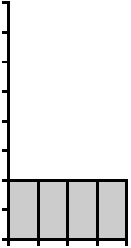
\includegraphics[width=20\unitlength]{bar1m}}
\cell{45}{5}{b}{\includegraphics[width=20\unitlength]{bar2m}}
\cell{75}{5}{b}{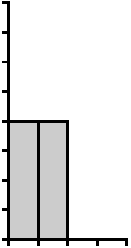
\includegraphics[width=20\unitlength]{bar3m}}
\cell{105}{5}{b}{\includegraphics[width=20\unitlength]{bar4m}}
\cell{5}{6}{r}{$\scriptstyle 0$}
\cell{5}{15.2}{r}{$\tfrac{1}{4}$}
\cell{5}{24.2}{r}{$\tfrac{1}{2}$}
\cell{5}{33.5}{r}{$\tfrac{3}{4}$}
\cell{5}{42.2}{r}{$\scriptstyle 1$}
\cell{35}{6}{r}{$\scriptstyle 0$}
\cell{35}{15.2}{r}{$\tfrac{1}{4}$}
\cell{35}{24.2}{r}{$\tfrac{1}{2}$}
\cell{35}{33.5}{r}{$\tfrac{3}{4}$}
\cell{35}{42.2}{r}{$\scriptstyle 1$}
\cell{65}{6}{r}{$\scriptstyle 0$}
\cell{65}{15.2}{r}{$\tfrac{1}{4}$}
\cell{65}{24.2}{r}{$\tfrac{1}{2}$}
\cell{65}{33.5}{r}{$\tfrac{3}{4}$}
\cell{65}{42.2}{r}{$\scriptstyle 1$}
\cell{95}{6}{r}{$\scriptstyle 0$}
\cell{95}{15.2}{r}{$\tfrac{1}{4}$}
\cell{95}{24.2}{r}{$\tfrac{1}{2}$}
\cell{95}{33.5}{r}{$\tfrac{3}{4}$}
\cell{95}{42.2}{r}{$\scriptstyle 1$}
% 
\cell{8.5}{4.5}{c}{$\scriptstyle 1$}
\cell{13}{4.5}{c}{$\scriptstyle 2$}
\cell{17.5}{4.5}{c}{$\scriptstyle 3$}
\cell{22}{4.5}{c}{$\scriptstyle 4$}
\cell{38.5}{4.5}{c}{$\scriptstyle 1$}
\cell{43}{4.5}{c}{$\scriptstyle 2$}
\cell{47.5}{4.5}{c}{$\scriptstyle 3$}
\cell{52}{4.5}{c}{$\scriptstyle 4$}
\cell{68.5}{4.5}{c}{$\scriptstyle 1$}
\cell{73}{4.5}{c}{$\scriptstyle 2$}
\cell{77.5}{4.5}{c}{$\scriptstyle 3$}
\cell{82}{4.5}{c}{$\scriptstyle 4$}
\cell{98.5}{4.5}{c}{$\scriptstyle 1$}
\cell{103}{4.5}{c}{$\scriptstyle 2$}
\cell{107.5}{4.5}{c}{$\scriptstyle 3$}
\cell{112}{4.5}{c}{$\scriptstyle 4$}
% 
\cell{-1.5}{24}{c}{\rotatebox{90}{Probability}}
% \cell{116.5}{24}{c}{\rotatebox{90}{probability}}
% 
\cell{15}{-1.5}{b}{Entropy: $2$}
\cell{45}{-2}{b}{Entropy: $1\tfrac{3}{4}$}
\cell{75}{-1.5}{b}{Entropy: $1$}
\cell{105}{-1.5}{b}{Entropy: $0$}
\end{picture}
\caption{Four probability distributions on $\{1, 2, 3, 4\}$, and their
  entropies to base~$2$.}  \lbl{fig:four-four-two}
\end{figure}

\begin{examples}
\lbl{egs:ent-ufm}
Figure~\ref{fig:four-four-two} shows the base~$2$ entropies $\Hi(\p)$ of
four distributions $\p \in \Delta_4$.  For instance, the second is computed
as 
% 
\begin{align*}
\Hi\Bigl(\tfrac{1}{2}, \tfrac{1}{4}, \tfrac{1}{8}, \tfrac{1}{8}\Bigr)     &
=
\tfrac{1}{2} \log_2 2 + \tfrac{1}{4} \log_2 4 
+ \tfrac{1}{8} \log_2 8 + \tfrac{1}{8} \log_2 8 
% \\
% &
% =
% \tfrac{1}{2} + \tfrac{2}{4} + \tfrac{3}{8} + \tfrac{3}{8}
=
1 \tfrac{3}{4}.
\end{align*}
% 
These examples illustrate the interpretation of entropy as uniformity.  The
highest entropy belongs to the first, uniform, distribution.  Each of the
four distributions on $\{1, 2, 3, 4\}$ is less uniform than its
predecessor, and, correspondingly, has lower entropy.
\end{examples}

We now set out the basic properties of entropy.  Here and later, we will
repeatedly use the following elementary fact about logarithms.

\begin{lemma}
\lbl{lemma:log-concave}
Let $\p \in \Delta_n$ and $x_1, \ldots, x_n \in (0, \infty)$.  Then
\[
\log \Biggl( \sum_{i = 1}^n p_i x_i \Biggr)
\geq
\sum_{i = 1}^n p_i \log x_i,
\]
with equality if and only if $x_i = x_j$ for all $i, j \in \supp(\p)$.
\end{lemma}

\begin{proof}
The function $\log \from (0, \infty) \to \R$ is strictly
concave\index{concavity}, since 
$\tfrac{d^2}{dx^2} \log x = -1/x^2 < 0$.  The result follows. 
\end{proof}

We now show that among all probability distributions on a finite set,
entropy is maximized by the uniform distribution and minimized by any
distribution of the form $(0, \ldots, 0, 1, 0, \ldots, 0)$.  

\begin{lemma}
\lbl{lemma:ent-max-min}
Let $n \geq 1$.
% 
\begin{enumerate}
\item 
\lbl{part:ent-min}
$H(\p) \geq 0$ for all $\p \in \Delta_n$, with equality if and only if $p_i
  = 1$ for some $i \in \{1, \ldots, n\}$. 

\item
\lbl{part:ent-max}
$H(\p) \leq \log n$ for all $\p \in \Delta_n$, with equality if and only if
  $\p = \vc{u}_n$.
\end{enumerate}
\end{lemma}

\begin{proof}
Part~\bref{part:ent-min} follows from the fact that $\log(1/p_i) \geq 0$
for all $i \in \supp(\p)$, with equality if and only if $p_i = 1$.
For~\bref{part:ent-max}, Lemma~\ref{lemma:log-concave} gives
\[
H(\p)
=
\sum_{i \in \supp(\p)} p_i \log \frac{1}{p_i}
\leq
\log \Biggl( \sum_{i \in \supp(\p)} p_i \cdot \frac{1}{p_i} \Biggr)
=
\log\mg{\supp(\p)}
\leq
\log n.
\]
Again by Lemma~\ref{lemma:log-concave}, the first inequality is an equality
if and only if $\p$ is uniform on its support.  The second inequality is an
equality if and only if $\p$ has full support.  The result follows.
\end{proof}

It is often useful to express entropy in terms of the 
function
\[
\partial \from [0, 1] \to \R
\ntn{partial}
\]
defined by
% 
\begin{equation}
\lbl{eq:defn-par}
\partial(x)
=
\begin{cases}
-x \log x       &\text{if } x > 0,      \\
0               &\text{if } x = 0.
\end{cases}
\end{equation}
% 
Thus,
% 
\begin{equation}
\lbl{eq:sh-par}
H(\p) = \sum_{i = 1}^n \partial(p_i)
\end{equation}
% 
for all $n \geq 1$ and $\p \in \Delta_n$.  

\begin{lemma}
\lbl{lemma:ent-cts}
For each $n \geq 1$, the entropy function $H \from \Delta_n \to \R$ is
continuous. 
\end{lemma}

\begin{proof}
This follows from equation~\eqref{eq:sh-par} and the elementary fact
that $\partial$ is continuous.
\end{proof}

The operator $\partial$ is a nonlinear derivation\index{derivation}:
% 
\begin{lemma}
\lbl{lemma:derivation}
$\partial(xy) = \partial(x)y + x\partial(y)$ for all $x, y \in [0, 1]$.
\qed
\end{lemma}

\begin{remark}
Up to a constant factor, $\partial$ is the only measurable function $d
\from [0, 1] \to \R$ satisfying $d(xy) = d(x)y + xd(y)$ for all $x, y$.
Indeed, taking $x = y = 0$ forces $d(0) = 0$, and the result follows
by applying Corollary~\ref{cor:cauchy-log-01} to the function $x \mapsto
d(x)/x$ on $(0, 1]$.
\end{remark}

We use Lemma~\ref{lemma:derivation} to prove the most important algebraic
property of Shannon entropy:

\begin{propn}[Chain rule]
\lbl{propn:ent-chain}
\index{chain rule!Shannon entropy@for Shannon entropy}
% 
Let $\vc{w} \in \Delta_n$ and $\p^1 \in \Delta_{k_1}, \ldots, \p^n \in
\Delta_{k_n}$.  Then
\[
H\bigl(\vc{w} \of (\p^1, \ldots, \p^n)\bigr)
=
H(\vc{w}) + \sum_{i = 1}^n w_i H(\p^i).
\]
\end{propn}

\begin{proof}
Writing $\p^i = \bigl(p^i_1, \ldots, p^i_{k_i}\bigr)$ and using
Lemma~\ref{lemma:derivation}, we have
% 
\begin{align*}
H\bigl(\vc{w} \of (\p^1, \ldots, \p^n)\bigr)    &
=
\sum_{i = 1}^n \sum_{j = 1}^{k_i} \partial \bigl(w_i p^i_j\bigr)   \\
&
=
\sum_{i} \sum_{j}
\bigl(\partial(w_i) p^i_j + w_i \partial\bigl(p^i_j\bigr)\bigr)   \\
&
=
\sum_{i} \partial(w_i) 
+
\sum_{i} w_i 
\sum_{j} \partial\bigl(p^i_j\bigr) \\
&
=
H(\vc{w}) + \sum_i w_i H(\p^i),
\end{align*}
% 
as required.
\end{proof}

\begin{example}
\index{coin!die-card@-die-card process}
% 
Consider again the coin-die-card process of Example~\ref{eg:comp-coin}.
How much information do we expect to gain from observing the final outcome
of the process?

Let us measure information by base~$2$ entropy, in bits.  The information
gained is as follows.
% 
\begin{itemize}
\item
Whether the final outcome is a number between~1 and~6 or a card tells us
whether the coin came up heads or tails.  This gives us $\Hi(\vc{u}_2) = 1$
bit of information.

\item
With probability $1/2$, the outcome is the result of a die\index{die} roll,
which would give us $\Hi(\vc{u}_6) = \log_2 6$ bits of information.

\item
With probability $1/2$, the outcome is the result of a card%
%
\index{cards, playing} 
% 
draw, which would give us $\Hi(\vc{u}_{52}) = \log_2 52$ bits of
information. 
\end{itemize}
% 
Hence in total, the expected information gained from observing the outcome
of the composite process is
\[
\Hi(\vc{u}_2) + \hlf \Hi(\vc{u}_6) + \hlf \Hi(\vc{u}_{52})
=
1 + \hlf \log_2 6 + \hlf \log_2 52
\]
bits.  If we have reasoned correctly, this should be equal to the entropy
of the composite process, which is
\[
\Hi\bigl(\vc{u}_2 \of (\vc{u}_6, \vc{u}_{52})\bigr)
=
\Hi\Bigl(\underbrace{\tfrac{1}{12}, \ldots, \tfrac{1}{12}}_{6},
\underbrace{\tfrac{1}{104}, \ldots, \tfrac{1}{104}}_{52}\Bigr)
\]
bits.  The chain rule guarantees that these two numbers are, indeed, equal.
\end{example}

\begin{cor}
\lbl{cor:ent-log}
For all $\vc{w} \in \Delta_n$ and $\p \in \Delta_k$,
% 
\begin{equation}
\lbl{eq:ent-log}
H(\vc{w} \otimes \p) = H(\vc{w}) + H(\vc{p}).
\end{equation}
\end{cor}

\begin{proof}
Take $\p^1 = \cdots = \p^n = \p$ in the chain rule.  
\end{proof}

In other words, $H$ has the logarithmic property of converting products
into sums.  Indeed, in the special case $\vc{w} = \vc{u}_n$ and $\p =
\vc{u}_k$, we have $\vc{w} \otimes \p = \vc{u}_{nk}$, so
equation~\eqref{eq:ent-log} is precisely the characteristic property of
the logarithm,
\[
\log(nk) = \log n + \log k.
\]
In the general case, equation~\eqref{eq:ent-log} states that the amount of
information gained by observing the outcome of a pair of
\emph{independent} events is equal to the information gained from the first
plus the information gained from the second.

\begin{remark}
\lbl{rmk:ent-chain-simp}
With the understanding that $H$ is symmetric in its arguments, the
chain%
%
\index{chain rule!forms of}
%
rule as stated in Proposition~\ref{propn:ent-chain} is equivalent to the
superficially less general statement that
% 
\begin{equation}
\lbl{eq:ent-chain-simp1}
H\bigl(pw_1, (1 - p)w_1, w_2, \ldots, w_n\bigr)
=
H(\vc{w}) + w_1 H(p, 1 - p)
\end{equation}
% 
for all $p \in [0, 1]$ and $\vc{w} \in \Delta_n$.  This is the special case
$k_1 = 2$, $k_2 = \cdots = k_n = 1$ of Proposition~\ref{propn:ent-chain},
and is sometimes known as the \demph{recursivity}\index{recursivity} of entropy
(Definition~1.2.8 of Acz\'el and Dar\'oczy~\cite{AcDa}) or the
\demph{grouping%
%
\index{grouping rule} 
% 
rule} (Problem~4 of Chapter~2 of Cover and Thomas~\cite{CoTh1}).

The general chain rule of Proposition~\ref{propn:ent-chain} is also
equivalent to a different special case:
\begin{multline*}
H\bigl(wp_1, \ldots, wp_k, (1 - w)r_1, \ldots, (1 - w)r_\ell\bigr)
=\\
H(w, 1 - w) + w H(\p) + (1 - w) H(\vc{r})
\end{multline*}
for all $w \in [0, 1]$, $\p \in \Delta_k$, and $\vc{r} \in \Delta_\ell$.
This is the special case $n = 2$ of Proposition~\ref{propn:ent-chain}.

Both equivalences are routine inductions, carried out in
Appendix~\ref{sec:chain}.
% Figure~\ref{fig:comp-trees} illustrates the
% types of composition used in the two special cases.
\end{remark}


\section{Entropy in terms of coding}
\lbl{sec:ent-coding}
\index{entropy!coding@via coding}


The theory of coding provides a very concrete way of understanding the
concept of information.  The fundamental concepts and theorems of coding
theory were set out in Shannon's%
%
\index{Shannon, Claude} 
% 
original 1948 paper~\cite{ShanMTC}, with rigour and detail added soon
afterwards by researchers such as Khinchin~\cite{Khin} and
Feinstein~\cite{Fein}.  This section presents parts of that early work, and
in particular, Shannon's source coding theorem.

The source%
% 
\index{Shannon, Claude!source coding theorem}
% 
coding theorem can be described informally as follows.  Take an alphabet of
symbols, say the English%
%
\index{English language} 
% 
letters \as{a} to \as{z}, which occur with known frequencies $p_1, \ldots,
p_{26}$.  We want to design a scheme that encodes each letter as a finite
sequence of $0$s and $1$s.  Using this system, any message in English can
also be encoded as a sequence of $0$s and $1$s, by concatenating the codes
for the letters in the message.  Of course, we want our coding scheme to
have the property that the encoded message can be decoded unambiguously,
and it is also natural to want it to use as few bits as possible.  Roughly
speaking, the theorem is that in the most efficient coding scheme, the
number of bits needed per symbol is the base~$2$ entropy of the frequency
distribution $\p$.

We now give a more precise account.  In this section, entropy will always
be taken to base~$2$.  Details of everything that follows can be found in
introductions to information theory such as Cover and Thomas (\cite{CoTh1},
Chapter~5), MacKay (\cite{MacKITI}, Chapter~4), and Jones and
Jones~\cite{JoJo}.

Take an alphabet of $n$ symbols, with frequency distribution $\p \in
\Delta_n$; thus, in messages written using this alphabet, we expect the
symbols to be used in proportions $p_1, \ldots, p_n$.  A
\demph{code}\index{code} is an assignment to each $i \in \{1, \ldots, n\}$
of a finite sequence of bits (a \demph{code word}).  The $i$th code word
is, then, an element of the set $\{0, 1\}^{L_i}$ for some integer $L_i \geq
0$, and $L_i$ is called the \demph{word%
%
\index{word length}
%
length} of the $i$th symbol.  The expected word length of a symbol in our
alphabet is
\[
\sum_{i = 1}^n p_i L_i.
\]
We seek a code that minimizes the average word length, subject to the
natural constraint of unambiguous decodability (made precise shortly).

\begin{example}
\lbl{eg:code-naive}
Take an alphabet of four symbols \as{a}, \as{b}, \as{c}, \as{d}, with
frequency distribution $\p = (1/2, 1/4, 1/8, 1/8)$.  How should we encode
our symbols as strings of bits, in a way that uses as few bits as possible?

The basic principle is that common symbols should have short code words.
(The same principle guided the design of Morse%
%
\index{Morse code} 
% 
code, where the most common letter, \as{e}, is encoded as a single dot, and
uncommon letters such as \as{z} use four dots or dashes.)  So let us encode
as follows:
\[
\as{a}: 0,
\quad
\as{b}: 10,
\quad
\as{c}: 110,
\quad
\as{d}: 111.
\]
For instance, 11110011010 represents \as{dbacb}.  The average word length
is
\[
\tfrac{1}{2} \cdot 1 +
\tfrac{1}{4} \cdot 2 + 
\tfrac{1}{8} \cdot 3 + 
\tfrac{1}{8} \cdot 3
=
1\tfrac{3}{4}.
\]
This is more efficient than the most naive coding system, which would
simply assign the four two-bit strings $00, 01, 10, 11$ to the four
symbols, for an average word length of $2$. 
\end{example}

A code is \demph{instantaneous}%
%
\index{instantaneous code} 
%
if none of the code words is a prefix (initial segment) of any other.
Thus, if $\delta_1 \cdots \delta_\ell$ and $\epsln_1 \cdots \epsln_m$ are
code words in an instantaneous code, with $\ell \leq m$, then $(\delta_1,
\ldots, \delta_\ell) \neq (\epsln_1, \ldots, \epsln_\ell)$.
% 
This is the non-ambiguity condition, guaranteeing that any string of bits
produced by the system can only be decoded in one possible way.  

\begin{example}
The code of Example~\ref{eg:code-naive} is instantaneous.  But if we changed
the code word for \as{b} to $11$, the code would no longer be
instantaneous, since $11$ is a prefix of the code words for both \as{c} and
\as{d}.  Messages in this new code are not uniquely decodable; for
instance, the string $110$ could be decoded as either \as{c} or \as{ba}.
\end{example}

The average word length $1\tfrac{3}{4}$ of the code in
Example~\ref{eg:code-naive} happens to be equal to the entropy of the
frequency distribution of the symbols, calculated in
Example~\ref{egs:ent-ufm}.  In fact, it is not possible to find an
instantaneous code whose average word length is any shorter.  This is an
instance of part~\bref{part:sh1-nogo-bound} of the following result.

\begin{propn}
\lbl{propn:sh1-nogo}
Let $n, L_1, \ldots, L_n \geq 1$, and suppose that there exists an
instantaneous code on the alphabet $\{1, \ldots, n\}$ with word lengths
$L_1, \ldots, L_n$.  Then:
% 
\begin{enumerate}
\item
\lbl{part:sh1-nogo-kraft}
$\displaystyle \sum_{i = 1}^n (1/2)^{L_i} \leq 1$;

\item
\lbl{part:sh1-nogo-bound}
$\displaystyle \sum_{i = 1}^n p_i L_i \geq \Hi(\p)$ for all $\p \in
\Delta_n$. 
\end{enumerate}
\end{propn}

Part~\bref{part:sh1-nogo-kraft}, together with
part~\bref{part:sh1-go-kraft} of Proposition~\ref{propn:sh1-go} below, is
known as \demph{Kraft's%
%
\index{Kraft's inequality} 
% 
inequality} (Theorem~5.2.1 of Cover and Thomas~\cite{CoTh1}, for instance).

\begin{proof}
To prove~\bref{part:sh1-nogo-kraft}, we consider binary expansions $0.b_1
b_2 \ldots$ of elements of $[0, 1)$, where $b_i \in \{0, 1\}$.  We make the
convention that if $x \in [0, 1)$ has two binary expansions, one ending
with an infinite sequence of $0$s and the other with an infinite
sequence of $1$s, we choose the former.  In this way, each $x \in [0,
1)$ determines an infinite sequence of bits $b_1, b_2, \ldots$

Take an instantaneous code with word lengths $L_1, \ldots, L_n$.
For $i \in \{1, \ldots, n\}$, write 
\[
J_i 
=
\bigl\{ x \in [0, 1) \such \text{the binary expansion of } x
\text{ begins with the $i$th code word} \bigr\}.
\]
Then $J_i$ is a half-open interval of length $(1/2)^{L_i}$.  Since the code
is instantaneous, the intervals $J_1, \ldots, J_n$ are disjoint.  But since
they are all subsets of $[0, 1)$, their total length is at most $1$, giving
the desired inequality.

For~\bref{part:sh1-nogo-bound}, let $\p \in \Delta_n$.  By
Lemma~\ref{lemma:log-concave} and part~\bref{part:sh1-nogo-kraft}, 
% 
\begin{align*}
\Hi(\p) - \sum_{i = 1}^n p_i L_i        &
=
\sum_{i \in \supp(\p)} p_i
\Bigl( \log_2 (1/p_i)
+ \log_2 \bigl((1/2)^{L_i} \bigr) \Bigr)   \\
&
=
\sum_{i \in \supp(\p)} 
p_i \log_2 \frac{(1/2)^{L_i}}{p_i}      \\
&
\leq
\log_2 \Biggl( 
\sum_{i \in \supp(\p)} p_i \cdot \frac{(1/2)^{L_i}}{p_i} 
\Biggr) \\
&
\leq
\log_2 \sum_{i = 1}^n (1/2)^{L_i}  \\
& 
\leq 
\log_2 1 = 0,
\end{align*}
% 
as required.
\end{proof}

The frequency distribution of Example~\ref{eg:code-naive} has the
exceptional property that all the frequencies are powers of $1/2$.
In such cases, it is always possible to find an instantaneous code in which
the $i$th symbol is encoded in $\log_2(1/p_i)$ bits, so that the average
word length is exactly the entropy.  In the general case, this is not quite
possible; but it is nearly possible, as follows.

\begin{propn}
\lbl{propn:sh1-go}
Let $\p \in \Delta_n$.  Then:
% 
\begin{enumerate}
\item 
\lbl{part:sh1-go-kraft}
there is an instantaneous code with word lengths $\lceil \log_2(1/p_1)
\rceil$, \ldots, $\lceil \log_2(1/p_n) \rceil$;

\item
\lbl{part:sh1-go-bound}
any such code has expected word length strictly less then
$\Hi(\p) + 1$.  
\end{enumerate}
\end{propn}

Here $\lceil x \rceil$ denotes the smallest integer greater than or equal
to $x$.  Codes with the property in~\bref{part:sh1-go-kraft} are called
\demph{Shannon%
%
\index{Shannon, Claude!code}
%
codes}.

\begin{proof}
For~\bref{part:sh1-go-kraft}, suppose without loss of generality that $p_1
\geq \cdots \geq p_n$.  For each $i \in \{1, \ldots, n\}$, put 
\[
L_i
=
\lceil \log_2(1/p_i) \rceil,
\quad
q_i 
=
(1/2)^{L_i}.
\]
In other words, $q_i$ is maximal among all powers of $1/2$ less than or
equal to $p_i$.  Now, $q_1, \ldots, q_i$ are all integer multiples of
$(1/2)^{L_i}$, so $q_1 + \cdots + q_{i - 1}$ and $q_1 + \cdots + q_i$ are
integer multiples of $(1/2)^{L_i}$ too.  It follows that the binary
expansions of the elements of the interval
\[
J_i = [q_1 + \cdots + q_{i - 1}, q_1 + \cdots + q_{i - 1} + q_i)
\]
all begin with the same $L_i$ bits, and, moreover, that no other element of
$[0, 1)$ begins with this bit-sequence.  (Here we use the same convention on
binary expansions as in the proof of Proposition~\ref{propn:sh1-nogo}.)
Take the $i$th code word to be this bit-sequence.  Since the intervals
$J_1, \ldots, J_n$ are disjoint, none of the code words is a prefix of any
other; that is, the code is instantaneous.

For~\bref{part:sh1-go-bound}, take a code as in~\bref{part:sh1-go-kraft},
again writing $L_i = \lceil \log_2(1/p_i)\rceil$.  We have
\[
L_i < \log_2(1/p_i) + 1
\]
for each $i \in \{1, \ldots, n\}$, so
\[
\sum_{i = 1}^n p_i L_i
=
\sum_{i \in \supp(\p)} p_i L_i
<
\sum_{i \in \supp(\p)} p_i \bigl( \log_2(1/p_i) + 1 \bigr)
=
\Hi(\p) + 1,
\]
as required.
\end{proof}

\begin{example}
Take the alphabet consisting of \as{a}, \as{b}, \as{c}, \as{d} with
frequencies $\p = (0.4, 0.3, 0.2, 0.1)$.  Following the construction in the
proof of Proposition~\ref{propn:sh1-go}, we round each frequency down to
the next power of $1/2$, giving
\[
(q_1, q_2, q_3, q_4)
=
\Bigl(\tfrac{1}{4}, \tfrac{1}{4}, \tfrac{1}{8}, \tfrac{1}{16}\Bigr)
=
\biggl( \Bigl(\tfrac{1}{2}\Bigr)^2, 
\Bigl(\tfrac{1}{2}\Bigr)^2, 
\Bigl(\tfrac{1}{2}\Bigr)^3, 
\Bigl(\tfrac{1}{2}\Bigr)^4 
\biggr).
\]
Thus, $(L_1, L_2, L_3, L_4) = (2, 2, 3, 4)$ and the intervals $J_i$ are as
follows, in binary notation:
% 
\begin{align*}
J_1     &
=
\Bigl[0, \tfrac{1}{4}\Bigr)     
=
[0.00, 0.01),   \\
J_2     &
=
\Bigl[\tfrac{1}{4}, \tfrac{1}{2}\Bigr)     
=
[0.01, 0.10),   \\
J_3     &
=
\Bigl[\tfrac{1}{2}, \tfrac{5}{8}\Bigr)     
=
[0.100, 0.101),   \\
J_4     &
=
\Bigl[\tfrac{5}{8}, \tfrac{11}{16}\Bigr)     
=
[0.1010, 0.1011).
\end{align*}
% 
We therefore encode as follows:
\[
\as{a}: 00,
\quad
\as{b}: 01, 
\quad
\as{c}: 100,
\quad
\as{d}: 1010.
\]
Short calculations show that
\[
\sum_{i = 1}^4 p_i L_i
=
2.4 
< 
2.846\ldots
=
\Hi(\p) + 1,
\]
as the proof of Proposition~\ref{propn:sh1-go} guarantees.

This is not the most efficient code. For instance, we could have encoded
\as{d} as 101 for a smaller average word length.  There are in fact
algorithms that construct for each $\p$ a code with the least possible
average word length, such as that of Huffman~\cite{Huff}%
%
\index{Huffman code}.  
% 
But we will not need such precision here.
\end{example}

\begin{example}
Similarly, the code in Example~\ref{eg:code-naive} is the one constructed
by the algorithm in the proof of Proposition~\ref{propn:sh1-go}.
\end{example}

\begin{remark}
The bound $\Hi(\p) + 1$ in Proposition~\ref{propn:sh1-go} cannot be
improved to $\Hi(\p) + c$ for any constant $c < 1$.  For instance, if a
two-symbol alphabet has frequency distribution $\p = (0.99, 0.01)$ then
$\Hi(\p) \approx \Hi(1, 0) = 0$ (since $\Hi$ is continuous), but clearly
the average word length cannot be reduced to below~$1$.
\end{remark}

We now state a version of Shannon's source coding theorem.

\begin{thm}[Shannon]%
\index{Shannon, Claude!source coding theorem}
% 
For an alphabet with frequency distribution $\p = (p_1, \ldots, p_n)$,
\[
\Hi(\p) \leq \inf \sum_{i = 1}^n p_i L_i < \Hi(\p) + 1,
\]
where the infimum is over all instantaneous codes on $n$ elements, with
$L_i$ denoting the $i$th word length.
\end{thm}

\begin{proof}
This is immediate from Propositions~\ref{propn:sh1-nogo}
and~\ref{propn:sh1-go}. 
\end{proof}

A crucial further insight of Shannon was that the upper bound $\Hi(\p) + 1$
can be reduced to $\Hi(\p) + \epsln$, for any $\epsln > 0$, as long as we
are willing to encode symbols in blocks\index{block} rather than one at a
time.  Informally, this works as follows.

For an alphabet with $n$ symbols, there are $n^{10}$ blocks of $10$
symbols.  Writing $\p \in \Delta_n$ for the frequency distribution of the
original alphabet and assuming that successive symbols in messages are
distributed independently, the frequency distribution of the $n^{10}$
blocks is $\p^{\otimes 10}$.  

Now treat each 10-symbol block as a unit, and consider ways of encoding
each block as a sequence of bits.  By Proposition~\ref{propn:sh1-go}, we
can find an instantaneous code for the blocks that uses an average of less
than $\Hi(\p^{\otimes 10}) + 1$ bits per block.  But $\Hi(\p^{\otimes 10})
= 10\Hi(\p)$ by Corollary~\ref{cor:ent-log}, so the average number of bits
per letter is less than
\[
\tfrac{1}{10} \Bigl( \Hi\bigl(\p^{\otimes 10}\bigr) + 1 \Bigr)
=
\Hi(\p) + \tfrac{1}{10}.
\]
In this way, by encoding symbols in large blocks rather than individually,
we can make the average number of bits per letter as close as we please to
the lower bound of $\Hi(\p)$.

(In applications, successive symbols are often not independent.  For
instance, in English, the letter pair \as{ch} is more frequent than
\as{hc}.  But it will follow from Remark~\ref{rmk:ub-coupling} that even if
they are not independent, the actual frequency distribution of the $n^{10}$
blocks has entropy at most $H(\p^{\otimes 10})$.  For that reason, the
argument above is valid even without the assumption of
independence.) 
\pagebreak

\begin{example}
Take a two-symbol alphabet \as{a}, \as{b} with frequency distribution $\p =
(0.6, 0.4)$.  Then $\Hi(\p) = 0.9709\ldots$\:\  We compute the average number
of bits per letter when encoding in larger and larger blocks, following the
code construction in the proof of Proposition~\ref{propn:sh1-go}.
% 
\begin{itemize}
\item 
First encode one symbol at a time.  We round each $p_i$ down to the next
power of $1/2$, giving $\bigl((1/2)^1,
(1/2)^2\bigr)$.  Hence the average number of bits per symbol is
\[
0.6 \times 1 + 0.4 \times 2 = 1.4.
\]

\item
Now encode symbols in blocks of two.  The frequency distribution of
\as{aa}, \as{ab}, \as{ba}, \as{bb} is $(0.36, 0.24, 0.24, 0.16)$ (assuming
that successive symbols are distributed independently).  Following the same
algorithm, we round down to $\bigl((1/2)^2, (1/2)^3,
(1/2)^3, (1/2)^3\bigr)$ and obtain an average of
\[
0.36 \times 2 + 0.24 \times 3 + 0.24 \times 3 + 0.16 \times 3
=
2.64
\]
bits per two-symbol block, or equivalently an average of $1.32$ bits per
symbol.  This is an improvement on the original code.

\item
Similarly, encoding in three-symbol blocks gives an average of
$1.117\ldots$ bits per symbol, which is closer still to the
ideal of $\Hi(\p) \approx 0.971$ bits per symbol.
\end{itemize}
% 
None of these three codes is as efficient as the naive code that assigns
the code words $0$ to \as{a} and $1$ to \as{b}, which has an average word
length of $1$.  But we can improve on that by encoding in large enough
blocks.  For instance, since
\[
0.971 + \tfrac{1}{35} < 1,
\]
we can attain an average word length of less than $1$ by coding blocks of
$35$ symbols at a time.
\end{example}

\begin{example}
\index{English language}
% 
In written English, the base~$2$ entropy of the frequency distribution of
the $26$~letters of the alphabet is approximately 4.1 (Section~2 of
Shannon~\cite{ShanPEP}).  Thus, by using sufficiently large blocks, one can
encode English using about four bits per letter.  (It is as if English had
only $2^{4.1} \approx 17$ letters, used with equal frequency.)  This is
without taking advantage of the fact that \as{ch} occurs more often than
\as{hc}, for instance.  Using the non-independence of neighbouring letters
would enable us to reduce the number of bits still further, as detailed by
Shannon~\cite{ShanPEP} and later researchers.
\end{example}

A convenient fiction\lbl{p:fiction} when reasoning about entropy is that
for every probability distribution $\p$, there is an instantaneous code
with average word length $\Hi(\p)$.  This is not true unless all the
nonzero frequencies happen to be powers of $\hlf$, but it is approximately
true in the sense just described: we can come arbitrarily close by encoding
in sufficiently large blocks.  Let us call this (usually nonexistent) code an
\demph{ideal\lbl{p:ideal}%
%
\index{ideal code} 
% 
code} for $\p$.

Ideal codes provide a way to understand the chain rule
(Proposition~\ref{propn:ent-chain}), as follows.

\begin{example}
\lbl{eg:ent-french}
\index{French language} 
% 
Consider again the French language (Example~\ref{eg:comp-french}), which is
written with symbols such as \as{\`a} made up of a letter (in this case,
\as{a}) and an accent (in this case, \as{\`{\:}}).
Figure~\ref{fig:ent-french} shows a hypothetical frequency distribution
$\vc{w}$ of the letters, hypothetical frequency distributions
\[
\p^1 \in \Delta_3, \ 
\p^2 \in \Delta_1, \
\ldots, \
\p^{26} \in \Delta_1
\]
of the accents on each letter, and the base~$2$ entropy of each of the
distributions $\vc{w}, \p^1, \ldots, \p^{26}$.

\begin{figure}
\centering
\lengths
\begin{picture}(120,53)(-4,-3.5)
\cell{55}{23}{c}{\includegraphics[height=42\unitlength]{accents_dotted_boxes}}
\cell{23}{22}{b}{\small 0.05}
\cell{41.5}{22}{b}{\small 0.02}
\cell{56}{22}{b}{\small 0.03}
\cell{102}{22}{b}{\small 0.004}
\cell{34}{27}{b}{\as{a}}
\cell{49}{27}{b}{\as{b}}
\cell{60}{27}{b}{\as{c}}
\cell{76}{27}{b}{$\cdots$}
\cell{92}{27}{b}{\as{z}}
% 
\cell{7.5}{10}{b}{\as{a}}
\cell{14.5}{10}{b}{\colorbox{white}{\as{\`a}\vphantom{$l^l$}}}
\cell{21}{10}{b}{\as{\^a}}
\cell{40}{10}{b}{\as{b}}
\cell{53}{10}{b}{\as{c}}
\cell{61}{9.3}{b}{\as{\c{c}}}
\cell{108.5}{10}{b}{\as{z}}
\cell{2}{5}{b}{\small0.5}
\cell{14.5}{5}{b}{\colorbox{white}{\small0.25\vphantom{$l^l$}}}
\cell{28}{5}{b}{\small0.25}
% \cell{28}{5}{b}{\small0.25}
% \cell{35.3}{5}{b}{\small0.25}
\cell{40}{5}{b}{\small1}
\cell{49.5}{5}{b}{\small0.5}
\cell{64.5}{5}{b}{\small0.5}
\cell{108.5}{5}{b}{\small1}
\cell{76}{9}{b}{$\cdots$}
% 
\cell{62.8}{45.5}{b}{Entropy $\Hi(0.05, 0.02, 0.03, \ldots, 0.004)$}
\cell{15.5}{0}{t}{Entropy $1.5$}
\cell{39}{0}{t}{Entropy $0$}
\cell{57}{0}{t}{Entropy $1$}
\cell{107}{0}{t}{Entropy $0$}
\end{picture}
\caption{The entropy of the French language
  (Example~\ref{eg:ent-french}).}
\lbl{fig:ent-french}
\end{figure}

To transmit a French symbol (such as \as{\`a}), we need to transmit both its
base letter (\as{a}) and its accent (\as{\`{\:}}).  Using ideal
codes, the average number of bits needed per symbol is as follows.  For
the base letter, we need $\Hi(\vc{w})$ bits.  The number of bits needed for
the accent depends on which letter it decorates:
% 
\begin{itemize}
\item 
with probability $w_1$, the letter is \as{a}, and then the average number
of bits needed for the accent is $\Hi(\p^1)$;

\item 
with probability $w_2$, the letter is \as{b}, and then the average number
of bits needed for the accent is $\Hi(\p^2)$;
\end{itemize}
% 
and so on.  Hence the average number of bits needed to encode the accent is
$\sum_{i = 1}^{26} w_i \Hi(\p^i)$.  The average number of bits needed per
symbol is the number for the base letter plus the number for the accent,
which is
% 
\begin{equation}
\lbl{eq:ent-french-cR}
\Hi(\vc{w}) + \sum_{i = 1}^{26} w_i \Hi(\p^i).
\end{equation}
% 
On the other hand, we saw in Example~\ref{eg:comp-french} that the overall
frequency distribution of the French symbols \as{a}, \as{\`a}, \as{\^a},
\as{b}, \ldots, \as{z} is $\vc{w} \of (\p^1, \ldots, \p^n)$, whose ideal
code uses
% 
\begin{equation}
\lbl{eq:ent-french-cL}
\Hi\bigl(\vc{w} \of (\p^1, \ldots, \p^n)\bigr)
\end{equation}
% 
bits per symbol.  If we have reasoned correctly then the
expressions~\eqref{eq:ent-french-cR} and~\eqref{eq:ent-french-cL} should be
equal.  The chain rule states that, indeed, they are.
\end{example}


\section{Entropy in terms of diversity}
\lbl{sec:ent-div}
\index{entropy!diversity@via diversity}

Entropies of various kinds have been used to measure biological diversity
for almost as long as diversity measures have been considered.  For
instance, among all the measures of diversity used by ecologists, one of the
most common is the Shannon entropy $H(\p)$.  Here $\p = (p_1, \ldots, p_n)$
is the relative abundance distribution of the community concerned, as in
Example~\ref{eg:prob-eco}.  For reasons that will be explained, when it
comes to measuring diversity, it is better to use the \emph{exponential} of
entropy than entropy itself.

Let us begin by considering intuitively what it means for a community of
$n$ species to be diverse, for a fixed value of $n$.  As described in the
Introduction, there is a spectrum of viewpoints on what the word
`diversity' should mean.  Loosely, though, diversity is low when most of
the population is concentrated into one or two very common species, and
high when the population is spread evenly across all species.  Another way
to say this is that diversity is low when an individual chosen at random
usually belongs to a common species, and high when an individual chosen at
random usually belongs to a rare species.  So, the diversity of
a community can be understood as the average rarity of an individual
belonging to it.

Since $p_i$ represents the relative abundance of the $i$th species, $1/p_i$
is a measure of its rarity\index{rarity} or specialness\index{specialness}.
We want to take the average rarity, and for now we will use the geometric
mean as our notion of average.  (Later, we will use different notions of
average.  The most important are the power means, which are introduced in
Section~\ref{sec:pwr-mns} and include the geometric mean.)  Thus, one
reasonable measure of the diversity of a community is the geometric mean of
the species rarities $1/p_1, \ldots, 1/p_n$, weighted by the species sizes
$p_1, \ldots, p_n$:
\[
\Biggl( \frac{1}{p_1} \Biggr)^{p_1}
\cdots
\Biggl( \frac{1}{p_n} \Biggr)^{p_n}.
\]
We therefore make the following definition.

\begin{defn}
\lbl{defn:div1}
\index{diversity!order 1@of order 1}
% 
Let $n \geq 1$ and $\p \in \Delta_n$.  The \demph{diversity of order~$1$}
of $\p$ is 
\[
D(\p)
=
\frac{1}{p_1^{p_1} p_2^{p_2} \cdots p_n^{p_n}},
\ntn{D}
\]
with the convention that $0^0 = 1$.
\end{defn}

Equivalently,
\[
D(\p)
=
\prod_{i \in \supp(\p)} p_i^{-p_i}
=
e^{H(\p)}.
\]
In short: diversity is the exponential of entropy.

\begin{remarks}
\begin{enumerate}
\item
The meaning of `order~$1$' will be revealed in Section~\ref{sec:ren-hill}.
It is related to the different possible notions of average.  In this
section, `diversity' will always mean diversity of order~$1$.

\item
No choice of base is involved in the definition of $D$, in contrast to the
situation for $H$ (Remark~\ref{rmk:ent-base}).  For instance, $D(\p)$ is
equal to both $e^{H(\p)}$ and $2^{\Hi(\p)}$.
\end{enumerate}
\end{remarks}

Crucially, the word `diversity' refers only to the \emph{relative}, not
absolute, abundances.%
%
\index{abundance!relative vs.\ absolute}  
% 
If half of a forest\index{forest!fire} burns down, or if a patient loses
$90\%$ of their gut%
%
\index{gut microbiome}%
\index{microbial systems}
% 
bacteria, then it may be an
ecological or medical 
disaster; but assuming that the system is well-mixed, the diversity does
not change.  In the language of physics, diversity is an
intensive%
% 
\index{intensive quantity} 
% 
quantity
(like density or temperature) rather than an extensive%
% 
\index{extensive quantity} 
% 
quantity (like mass or heat), meaning that it is independent of the
system's size.

Lemma~\ref{lemma:ent-max-min} immediately implies:
% 
\begin{lemma}
\lbl{lemma:div1-max-min}
Let $n \geq 1$.
% 
\begin{enumerate}
\item 
\lbl{part:div1-min}
$D(\p) \geq 1$ for all $\p \in \Delta_n$, with equality if and only if $p_i
  = 1$ for some $i \in \{1, \ldots, n\}$. 

\item
\lbl{part:div1-max}
$D(\p) \leq n$ for all $\p \in \Delta_n$, with equality if and only if
  $\p = \vc{u}_n$.
\end{enumerate}
\qed
\end{lemma}

Similarly, the continuity of entropy (Lemma~\ref{lemma:ent-cts})
immediately implies:
% 
\begin{lemma}
\lbl{lemma:div1-cts}
For each $n \geq 1$, the diversity function $D \from \Delta_n \to \R$ of
order~$1$ is continuous.  
\qed
\end{lemma}

Evidently
\[
D(\vc{u}_n) = n 
\]
for all $n \geq 1$.  This is a very important property for a diversity
measure, and we adopt the standard terminology for it:

\begin{defn}
\lbl{defn:div-eff}
Let $\bigl( E \from \Delta_n \to (0, \infty) \bigr)_{n \geq 1}$ be a
sequence of functions.  Then $E$ is an \demph{effective%
%
\index{effective number} 
%
number} if
$E(\vc{u}_n) = n$ for all $n \geq 1$. 
\end{defn}

Thus, $D$ is an effective number.  When the species are all present in
equal quantities, we think of the community as containing $n$ fully
present species and assign it a diversity value of $n$.  On the other hand,
if one species accounts for nearly $100\%$ of the community and all the
others are very rare, then the diversity value is barely more than~$1$ (by
Lemmas~\ref{lemma:div1-max-min}\bref{part:div1-min}
and~\ref{lemma:div1-cts}).  Effectively, there is barely more than one
species present.

For instance, if a community has a diversity of $18.2$, then the community
is slightly more diverse than a community of $18$ equally abundant species.
There are `effectively' slightly more than $18$ balanced species.

\begin{examples}
\lbl{egs:div1-ufm}
For the four distributions on $\{1, 2, 3, 4\}$ in
Examples~\ref{egs:ent-ufm}, the diversities are
\[
2^2 = 4, 
\quad
2^{7/4} \approx 3.364,
\quad
2^1 = 2,
\quad
2^0 = 1,
\]
respectively.  In particular, the community represented by the second
distribution is judged by $D$ to be somewhat more diverse than a community
of three species in equal proportions, but less diverse than a balanced
community of four species.
\end{examples}

Despite the popularity of Shannon entropy as a measure of biological
diversity, many ecologists have argued that it should be rejected in favour
of its exponential, including MacArthur~\cite{MacA} in 1965, Buzas and
Gibson~\cite{BuGi} in 1969, and Whittaker~\cite{WhitEMS} in 1972.  More
recently and more generally, Jost~\cite{JostED,JostPDI,JostMBD} has argued
convincingly that when measuring diversity, we should only use effective
numbers.  (That principle appears to be gaining acceptance, judging by the
editorial~\cite{ElliPD} of Ellison.)  The following example is adapted from
Jost~\cite{JostPDI}.%
%
\index{Jost, Lou}

\begin{example}
\lbl{eg:plague}%
\index{plague}%
\index{diversity measure!logical behaviour of}
% 
Suppose that a plague strikes a continent of a million equally common
species, rendering $90\%$ of the species extinct and leaving the remaining
$10\%$ untouched.  How do $H$ and $D$ respond to this catastrophe?

The Shannon entropy $H$ drops by just
\[
1 - \frac{\log(10^5)}{\log(10^6)} = \frac{1}{6} \approx 17\%,
\]
suggesting a change of considerably smaller magnitude than the one that
actually occurred.  For comparison, if a community of four equally common
species loses only \emph{one} of its species, the rest remaining unchanged,
this causes a drop in Shannon entropy of
\[
1 - \frac{\log 3}{\log 4} \approx 21\%.
\]
So, if we judge by percentage change in Shannon entropy, losing $25\%$ of
four species destroys a greater proportion of the diversity than losing
$90\%$ of a million species.  Shannon entropy drops \emph{more} in the
situation where the species loss is \emph{less}.  So as an indicator of
change in diversity, percentage change in Shannon entropy is plainly
unsuitable. 

However, the effect of the plague on the diversity $D$ is to make it drop
by $90\%$ (from $10^6$ to $10^5$), because $D$ is an effective number.  And
for the same reason, in the four-species example, $D$ drops by $25\%$ (from
$4$ to $3$).  This is intuitively reasonable behaviour, faithfully
reflecting the scale of the change.
\end{example}

In information and coding theory, the logarithmic measure $H$ is the
more useful form, corresponding as it does to the number of bits per symbol
in an ideal code.  But for species diversity, it is the number of
species (not its logarithm) with which we reason most naturally.

We now consider the chain rule in terms of diversity.  Taking exponentials
in Proposition~\ref{propn:ent-chain} gives:

\begin{cor}
\lbl{cor:div1-chain}
Let $n, k_1, \ldots, k_n \geq 1$.  Then
\[
D\bigl(\vc{w} \of (\p^1, \ldots, \p^n)\bigr)
=
D(\vc{w}) \cdot \prod_{i = 1}^n D\bigl(\p^i\bigr)^{w_i}
\]
for all $\vc{w} \in \Delta_n$ and $\p^i \in \Delta_{k_i}$.
\qed
\end{cor}

The second factor on the right-hand side is the geometric mean of the
diversities $D(\p^1), \ldots, D(\p^n)$, weighted by $w_1, \ldots, w_n$.

The most important aspect of this result is not the specific formula, but
the fact that the diversity of the composite distribution depends only on
$\vc{w}$ and $D(\p^1), \ldots, D(\p^n)$, \emph{not} on $\p^1, \ldots, \p^n$
themselves.  This can be understood in either of the following ways.

\begin{example}
\lbl{eg:div1-chain-islands}
\index{islands!diversity of group of}
% 
As in Example~\ref{eg:comp-islands}, consider a group of $n$ islands of
relative sizes $w_1, \ldots, w_n$, with no species shared between islands.
Let $d_i$ denote $D(\p^i)$, the diversity of the $i$th island.  Then the
diversity of the whole island group is
% 
\begin{equation}
\lbl{eq:div1-chain-islands}
D(\vc{w}) \cdot d_1^{w_1} \cdots d_n^{w_n}.
\end{equation}
% 
Thus, the diversity of the whole island group is determined by the
diversities and relative sizes of the islands.  It can be computed without
reference to the population distributions on each island.  
\end{example}

\begin{example}
\lbl{eg:div1-chain-genus}
\index{genus}
% 
As in Example~\ref{eg:comp-genus}, consider a community of $n$ genera, with
the $i$th genus divided into $k_i$ species.  Let $\vc{w}$ denote the genus
distribution and $d_i$ the diversity of the species in the $i$th genus.
Then the species diversity of the whole community is again given
by~\eqref{eq:div1-chain-islands}.  For instance, if there are $2$~equally
abundant genera, with the first genus consisting of~$45$ species of equal
abundance and the second consisting of~$5$ species of equal abundance, then
the diversity of the whole community is
\[
D\bigl(\vc{u}_2 \of (\vc{u}_{45}, \vc{u}_5)\bigr)
=
D(\vc{u}_2) \cdot D(\vc{u}_{45})^{1/2} D(\vc{u}_5)^{1/2}
=
2 \sqrt{45}\sqrt{5} 
=
30.
\]
In other words, the whole community of $45 + 5 = 50$ species, which has
relative abundance distribution
\[
\Bigl(
\underbrace{\tfrac{1}{90}, \ldots, \tfrac{1}{90}}_{45},
\underbrace{\tfrac{1}{10}, \ldots, \tfrac{1}{10}}_{5}
\Bigr).
\]
has the same diversity as a community of~$30$ species of equal abundance.
\end{example}

Different chain rules will appear in Sections~\ref{sec:ren-hill}
and~\ref{sec:sim-props}, where we consider diversity of orders other
than~$1$.  But all share the crucial property that $D(\vc{w} \of (\p^1,
\ldots, \p^n))$ depends only on $\vc{w}$ and $D(\p^1), \ldots, D(\p^n)$.

We refer to this property of $D$ as
\demph{modularity}\lbl{p:D-mod}%
%
\index{modularity!diversity of order 1@of diversity of order 1}.  
%
The word is used here in the sense of modular software design, buildings or
furniture (as opposed to modular arithmetic or modules over a ring, say).
In this metaphor, the islands of Example~\ref{eg:div1-chain-islands} or the
genera of Example~\ref{eg:div1-chain-genus} are the `modules': when it
comes to computing the diversity of the whole assemblage, they are black
boxes whose internal features we do not need to know.

The logarithmic property of $H$ (Corollary~\ref{cor:ent-log}) translates
into a multiplicative property of $D$:
% 
\begin{equation}
\lbl{eq:div1-mult}
D(\vc{w} \otimes \vc{p}) = D(\vc{w}) \cdot D(\vc{p})
\end{equation}
% 
($n, k \geq 1$, $\vc{w} \in \Delta_n$, $\p \in \Delta_k$).  An important
special case is the \demph{replication\lbl{p:D-rep}%
% 
\index{replication principle!diversity of order 1@for diversity of order 1} 
% 
principle}:
\[
D(\vc{u}_n \otimes \p) = n D(\p)
\]
($n, k \geq 1$, $\p \in \Delta_k$).  In the language of
Example~\ref{eg:div1-chain-islands}, this principle states that given $n$
islands of equal size and the same species distributions, but with no
actual shared species, the diversity of the whole island group is $n$ times
the diversity of any individual island.

Another argument of Jost%
%
\index{Jost, Lou} 
%
(adapted from~\cite{JostMBD} and~\cite{JDWG}) makes a compelling case for
the importance of the replication principle:

\begin{example}
\index{oil company}%
\index{diversity measure!logical behaviour of}%
% 
\lbl{eg:oil} An oil company is planning to carry out work on a group of
islands that will destroy all wildlife on half of the islands.%
%
\index{islands!oil drilling on}
% 
Environmentalists are bringing a legal case to stop them.  What would be
the impact of the work on biodiversity?

Suppose that there are~$16$ equally-sized islands in the group, that there
are no species shared between islands, and that each island has diversity
$4$.  Then before the oil work, the diversity of the island group is
\[
16 \times 4 = 64.
\]
Afterwards, similarly, it will be $32$.  Thus, the diversity is reduced by
$50\%$.  This is intuitively reasonable, and is a consequence of the
replication principle for~$D$.

However, one of the most popular measures of diversity in ecology is
Shannon entropy (`many long-term investigations have chosen it as their
benchmark of biological diversity': Magurran~\cite{Magu},%
% 
\index{Magurran, Anne}
% 
p.~101).  The oil company's lawyers can therefore argue as follows.  Before
the works, the `diversity' (Shannon entropy) is $\log 64$, and afterwards,
it will be $\log 32$.  Thus, the proportion of diversity preserved is
\[
\frac{\log 32}{\log 64} 
% =
% \frac{\log_2 32}{\log_2 64}
=
\frac{5}{6} 
\approx
83\%.
\]
On the other hand, the environmentalists' lawyers can argue that the
islands whose wildlife is to be exterminated have a diversity of $\log
32$, out of a total of $\log 64$, so the proportion of diversity destroyed
will be 
\[
\frac{\log 32}{\log 64}
% =
% \frac{\log_2 32}{\log_2 64}
=
\frac{5}{6}
\approx 
83\%.
\]
So the oil company can truthfully claim that by the scientifically accepted
measure, $83\%$ of the diversity will be preserved, while the
environmentalists can just as legitimately claim that $83\%$ of the
diversity will be lost.  They cannot both be right, and, of course, both
are wrong: by any reasonable measure, $50\%$ of the diversity is preserved
and $50\%$ is lost.  The reason for the contradictory and illogical
conclusions is that Shannon entropy does not satisfy the replication
principle. 

Although this is an idealized hypothetical example, it is not hard to
see how a choice of diversity measure, far from being some obscure
theoretical issue, could have genuine environmental consequences.
\end{example}

Although the diversity measure $D$ does satisfy the replication principle,
and in that sense behaves logically, it has a glaring deficiency: it
takes no notice of the varying similarities%
%
\index{similarity!species@of species} 
% 
between species.  A forest consisting of ten equally abundant
species of larch is intuitively less diverse than a forest of ten equally
abundant but highly varied tree species.  However, the measure $D$ gives
the same diversity to both.  The same criticism can be levelled at most of
the diversity measures used in ecology, and a remedy is presented in
Chapter~\ref{ch:sim}.


\section{The chain rule characterizes entropy}
\lbl{sec:ent-chain}
\index{chain rule!Shannon entropy@for Shannon entropy}


There are many characterizations of Shannon entropy, beginning with one in
the original paper by Shannon%
%
\index{Shannon, Claude}
% 
himself (\cite{ShanMTC}, Theorem~2).  Here,
we prove a variant of one of the best-known such theorems, due
to Dmitry Faddeev~\cite{Fadd}.  

\begin{thm}[Faddeev]
\lbl{thm:faddeev}%
\index{Faddeev, Dmitry!entropy theorem}
% 
Let $( I \from \Delta_n \to \R )_{n \geq 1}$ be a sequence of
functions.  The following are equivalent:
% 
\begin{enumerate}
\item 
\lbl{part:faddeev-condns}
the functions $I$ are continuous and satisfy the chain rule
\[
I\bigl(\vc{w} \of (\p^1, \ldots, \p^n)\bigr)
=
I(\vc{w}) + \sum_{i = 1}^n w_i I(\p^i)
\]
($n, k_1, \ldots, k_n \geq 1$, $\vc{w} \in \Delta_n$, $\vc{p}^i \in
\Delta_{k_i}$);

\item
\lbl{part:faddeev-form}
$I = cH$ for some $c \in \R$.
\end{enumerate}
\end{thm}

In other words, up to a constant factor, entropy is uniquely characterized
by the chain rule and continuity.  We already know
that~\bref{part:faddeev-form} implies~\bref{part:faddeev-condns}; the
challenge is to show that~\bref{part:faddeev-condns}
implies~\bref{part:faddeev-form}. 

\begin{remarks}
\lbl{rmks:faddeev}
\begin{enumerate}
\item 
As noted in Remark~\ref{rmk:ent-base}, the appearance of the constant
factor should not be a surprise.  We could eliminate it by adding the axiom
that $I(\vc{u}_2) = \log 2$, for instance.

\item
\lbl{rmk:faddeev-sym} 
% \index{Faddeev, Dmitry!entropy theorem!role of symmetry in} 
\index{symmetry in Faddeev-type theorems}
% 
The theorem that Faddeev proved
in~\cite{Fadd} was slightly different.  He assumed that $I$ was symmetric,
that is, unchanged when the arguments $p_1, \ldots, p_n$ are permuted, but
he assumed only the superficially simpler form of the chain rule stated as
equation~\eqref{eq:ent-chain-simp1} (Remark~\ref{rmk:ent-chain-simp}).  As
noted in that remark, if we assume symmetry then the two forms
of the chain rule are equivalent via a straightforward induction
(Appendix~\ref{sec:chain}).  On the other hand, Theorem~\ref{thm:faddeev}
tells us that if we assume the chain rule in its general form then we do
not need symmetry.  This is not an obvious consequence of Faddeev's
original theorem.

\item
\lbl{rmk:faddeev-lee}
If we assume symmetry, the hypotheses of Faddeev's original theorem can be
weakened in a different direction, replacing
continuity by measurability.%
% 
\index{measurability!entropy@of entropy}
% 
This is a 1964 theorem of Lee~\cite{Lee}% 
%
\index{Lee, Pan-Mook}.
%
We return to Lee's theorem at the end of
Chapter~\ref{ch:p}, but omit the proof.  

\item
\lbl{rmk:faddeev-reg}
It is not possible to prove a Faddeev-type theorem with no regularity
conditions at all (unless one drops the axiom of choice).  Indeed, let $f
\from \R \to \R$ be an additive nonlinear function, as in
Remark~\ref{rmk:choice}.  Then the assignment
\[
\p \mapsto - \sum_{i \in \supp(\p)} p_i f(\log p_i)
\]
satisfies the chain rule but is not a scalar multiple of Shannon
entropy. 
\end{enumerate}
\end{remarks}

The remainder of this section is devoted to the proof of
Theorem~\ref{thm:faddeev}.  \femph{For the rest of this section}, let $(I
\from \Delta_n \to \R)_{n \geq 1}$ be a sequence of continuous functions
satisfying the chain rule.

The strategy of the proof is to show that $I$ is proportional to $H$ on
successively larger classes of probability distributions.  First we prove
it for the uniform distributions $\vc{u}_n$, using the results on
logarithmic sequences in Section~\ref{sec:log-seqs}.  This forms the bulk
of the proof.  It is then relatively easy to extend the result to
distributions $\p$ for which each $p_i$ is a positive rational number, and
from there, by continuity, to all distributions.

We begin by studying the real sequence $(I(\vc{u}_n))_{n \geq 1}$.

\begin{lemma}
\lbl{lemma:fad-log}
\begin{enumerate}
\item 
\lbl{part:fad-two}
$I(\vc{u}_{mn}) = I(\vc{u}_m) + I(\vc{u}_n)$ for all $m, n \geq 1$.

\item
\lbl{part:fad-zero}
$I(\vc{u}_1) = 0$.
\end{enumerate}
\end{lemma}

\begin{proof}
By the chain rule, $I$ has the logarithmic property
\[
I(\vc{w} \otimes \vc{p}) =
I\bigl(\vc{w} \of (\p, \ldots, \p)\bigr) =
I(\vc{w}) + I(\vc{p})
\]
($\vc{w} \in \Delta_m$, $\vc{p} \in \Delta_n$).  In particular,
for all $m, n \geq 1$,
\[
I(\vc{u}_{mn}) 
= 
I(\vc{u}_m \otimes \vc{u}_n) 
=
I(\vc{u}_m) + I(\vc{u}_n),
\]
proving~\bref{part:fad-two}.  For~\bref{part:fad-zero}, take $m = n = 1$
in~\bref{part:fad-two}.
\end{proof}

As we saw in Section~\ref{sec:log-seqs}, the property $I(\vc{u}_{mn}) =
I(\vc{u}_m) + I(\vc{u}_n)$ alone does not tell us very much about the
sequence $(I(\vc{u}_n))$.  To take advantage of the results in that
section, we will need to prove some analytic condition on the sequence.
Specifically, we will show that $I(\vc{u}_{n + 1}) - I(\vc{u}_n) \to 0$ as
$n \to \infty$, then apply Corollary~\ref{cor:erdos-lim}.
\pagebreak

\begin{lemma}
\lbl{lemma:fad-10}
$I(1, 0) = 0$.
\end{lemma}

\begin{proof}
We compute $I(1, 0, 0)$ in two ways.  On the one hand, using the chain rule,
\[
I(1, 0, 0)
=
I\Bigl((1, 0) \of \bigl((1, 0), \vc{u}_1\bigr)\Bigr)
=
I(1, 0) + 1 \cdot I(1, 0) + 0 \cdot I(\vc{u}_1)
=
2I(1, 0).
\]
On the other, using the chain rule again and the fact that $I(\vc{u}_1) = 0$,
\[
I(1, 0, 0)
=
I\Bigl((1, 0) \of \bigl(\vc{u}_1, (1, 0)\bigr)\Bigr)
=
I(1, 0) + 1 \cdot I(\vc{u}_1) + 0 \cdot I(1, 0)
=
I(1, 0).
\]
Hence $I(1, 0) = 0$.
\end{proof}

\begin{lemma}
\lbl{lemma:diff-nearly-zero}
$I(\vc{u}_{n + 1}) - \tfrac{n}{n + 1} I(\vc{u}_n) \to 0$ as $n \to \infty$.
\end{lemma}

\begin{proof}
We have
\[
\vc{u}_{n + 1} 
=
\biggl( \frac{n}{n + 1}, \frac{1}{n + 1} \biggr) \of (\vc{u}_n, \vc{u}_1),
\]
so by the chain rule and the fact that $I(\vc{u}_1) = 0$,
\[
I(\vc{u}_{n + 1})
=
I\biggl( \frac{n}{n + 1}, \frac{1}{n + 1} \biggr)
+
\frac{n}{n + 1} I(\vc{u}_n).
\]
Hence
\[
I(\vc{u}_{n + 1}) - \frac{n}{n + 1} I(\vc{u}_n)
=
I\biggl( \frac{n}{n + 1}, \frac{1}{n + 1} \biggr)
\to 
I(1, 0)
=
0
\]
as $n \to \infty$, by continuity and Lemma~\ref{lemma:fad-10}.
\end{proof}

Now we can use the results of Section~\ref{sec:log-seqs}.

\begin{lemma}
\lbl{lemma:sh-ent-u}
There exists a constant $c \in \R$ such that $I(\vc{u}_n) = cH(\vc{u}_n)$
for all $n \geq 1$.
\end{lemma}

\begin{proof}
By Lemma~\ref{lemma:fad-log}\bref{part:fad-two}, the sequence
$(I(\vc{u}_n))$ is logarithmic.  By Lemmas~\ref{lemma:diff-nearly-zero}
and~\ref{lemma:seq-improvement}, $\lim_{n \to \infty} \bigl( I(\vc{u}_{n +
  1}) - I(\vc{u}_n)\bigr) = 0$.  Hence by Corollary~\ref{cor:erdos-lim},
there is some $c \in \R$ such that for all $n \geq 1$,
\[
I(\vc{u}_n) 
=
c \log n
=
c H(\vc{u}_n).
\]
\end{proof}

We now move to the second phase of the proof of Theorem~\ref{thm:faddeev}.
Let $c$ be the constant of Lemma~\ref{lemma:sh-ent-u} (which is uniquely
determined).  

\begin{lemma}
\lbl{lemma:fad-rational}
Let $\p \in \Delta_n$ with $p_1, \ldots, p_n$ rational and nonzero.  Then
$I(\p) = cH(\p)$. 
\end{lemma}

\begin{proof}
We can write 
\[
\p = \biggl( \frac{k_1}{k}, \ldots, \frac{k_n}{k} \biggr)
\]
for some positive integers $k_1, \ldots, k_n$, where $k = k_1 + \cdots +
k_n$.  Then
\[
\p \of (\vc{u}_{k_1}, \ldots, \vc{u}_{k_n}) = \vc{u}_k.
\]
Since $I$ satisfies the chain rule and $I(\vc{u}_r) = cH(\vc{u}_r)$ for
all $r \geq 1$, we have
\[
I(\p) + \sum_{i = 1}^n p_i \cdot cH(\vc{u}_{k_i}) = cH(\vc{u}_k).
\]
But since $cH$ satisfies the chain rule too, we also have
\[
cH(\p) + \sum_{i = 1}^n p_i \cdot cH(\vc{u}_{k_i}) = cH(\vc{u}_k).
\]
The result follows.
\end{proof}

The third and final phase of the proof is trivial: since the probability
distributions with positive rational probabilities are dense in the space
$\Delta_n$ of all probability distributions, and since $I$ and $cH$
are continuous functions agreeing on this dense set, they are equal
everywhere.  This proves Theorem~\ref{thm:faddeev}.

Like any result on entropy, Faddeev's theorem can be translated into
diversity terms.  In the following corollary, we eliminate the arbitrary
constant factor by requiring that $E$ be an effective number.  

\begin{cor}
\lbl{cor:fad-div}
Let $\bigl( E \from \Delta_n \to (0, \infty) \bigr)_{n \geq 1}$ be a
sequence of functions.  The following are equivalent:
% 
\begin{enumerate}
\item 
\lbl{part:fad-div-condns}
the functions $E$ are continuous and satisfy the chain rule
% 
\begin{equation}
\lbl{eq:E-div-chain}
E\bigl(\vc{w} \of (\p^1, \ldots, \p^n)\bigr)
=
E(\vc{w}) \cdot \prod_{i = 1}^n E(\p^i)^{w_i}
\end{equation}
% 
($n, k_1, \ldots, k_n \geq 1$, $\vc{w} \in \Delta_n$, $\vc{p}^i \in
\Delta_{k_i}$), and $E$ is an effective number;

\item
\lbl{part:fad-div-form}
$E = D$.
\end{enumerate}
\end{cor}

\begin{proof}
By Faddeev's theorem applied to $\log E$, the sequences of continuous
functions $E$ satisfying the diversity chain rule~\eqref{eq:E-div-chain}
are exactly the real powers $D^c$ ($c \in \R$).  But the effective number
property (or indeed, the single equation $E(\vc{u}_2) = 2$) then forces $c
= 1$.
\end{proof}

